
\begin{frame}{‌الگوریتم کروسکال}
\begin{itemize}\itemr
\item[-]
الگوریتم کروسکال ابتدا به ازای هر رأس یک مجموعهٔ مجزا ایجاد می‌کند. سپس برای یافتن یال مطمئن در هر مرحله از بین همهٔ یال‌هایی که دو رأس در دو مجموعهٔ مجزا را به یکدیگر متصل می‌کنند، یال
\m{(u,v)}
با کمترین وزن را انتخاب می‌کند.
وقتی یال
\m{(u,v)}
به عنوان یک یال از درخت پوشای کمینه انتخاب شد،
مجموعه‌ای که رأس 
\m{u}
در آن قرار دارد به مجموعه‌ای که رأس 
\m{v}
در آن قرار دارد متصل می‌شوند.
%\item[-]
%فرض کنید
%\m{C_1}
%و
%\m{C_2}
%دو درخت باشند که با یال
%\m{(u,v)}
%به یکدیگر متصل شده‌اند. از آنجایی که
%\m{(u,v)}
%باید یک یال سبک باشد که
%\m{C_1}
%را به یک درخت دیگر متصل می‌کند،
%\m{(u,v)}
%یک یال مطمئن برای
%\m{C_1}
%است.
\item[-]
الگوریتم کروسکال یک الگوریتم حریصانه است زیرا در هرگام، یالی را اضافه می‌کند که کمترین وزن را دارد و در نهایت درخت به دست آمده دارای کمترین وزن خواهد بود.
\end{itemize}
\end{frame}



\begin{frame}{‌الگوریتم کروسکال}
\begin{itemize}\itemr
\item[-]
در شکل زیر روند اجرای الگوریتم کروسکال نشان داده شده است.
\begin{figure}
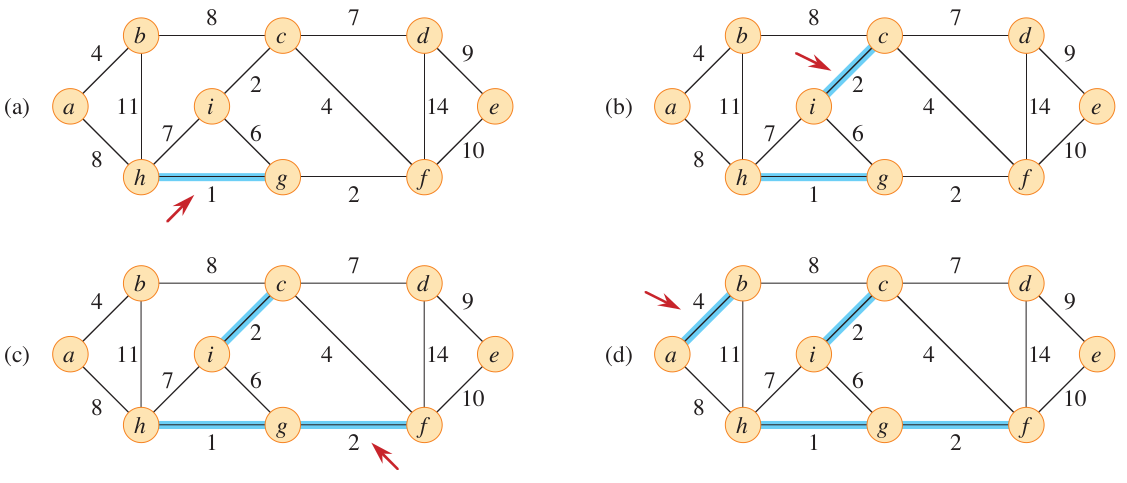
\includegraphics[width=0.7\textwidth]{figs/chap07/592-kruskal1}
\end{figure}
\end{itemize}
\end{frame}

\begin{frame}{‌الگوریتم کروسکال}
\begin{itemize}\itemr
\item[-]
\begin{figure}
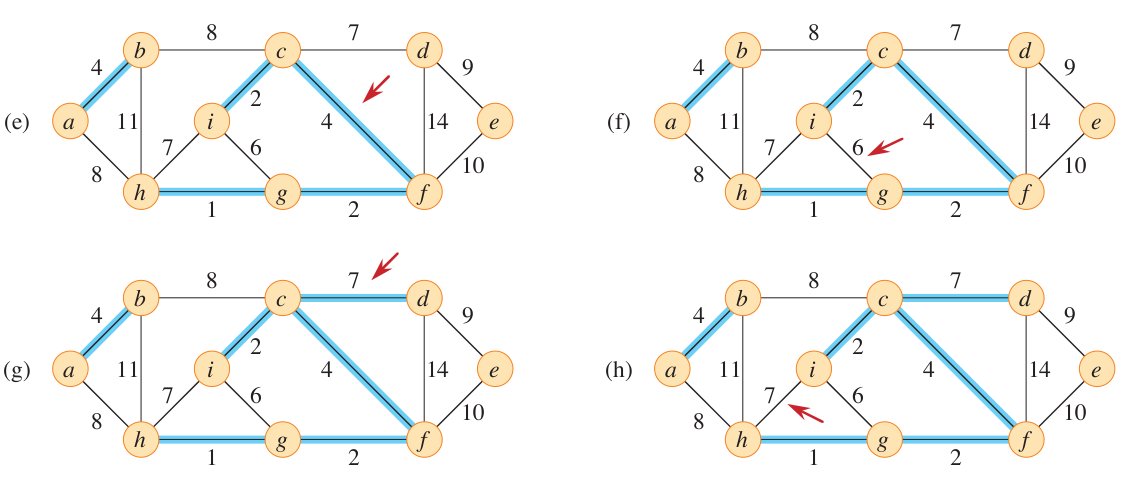
\includegraphics[width=0.7\textwidth]{figs/chap07/592-kruskal2}
\end{figure}
\end{itemize}
\end{frame}

\begin{frame}{‌الگوریتم کروسکال}
\begin{itemize}\itemr
\item[-]
\begin{figure}
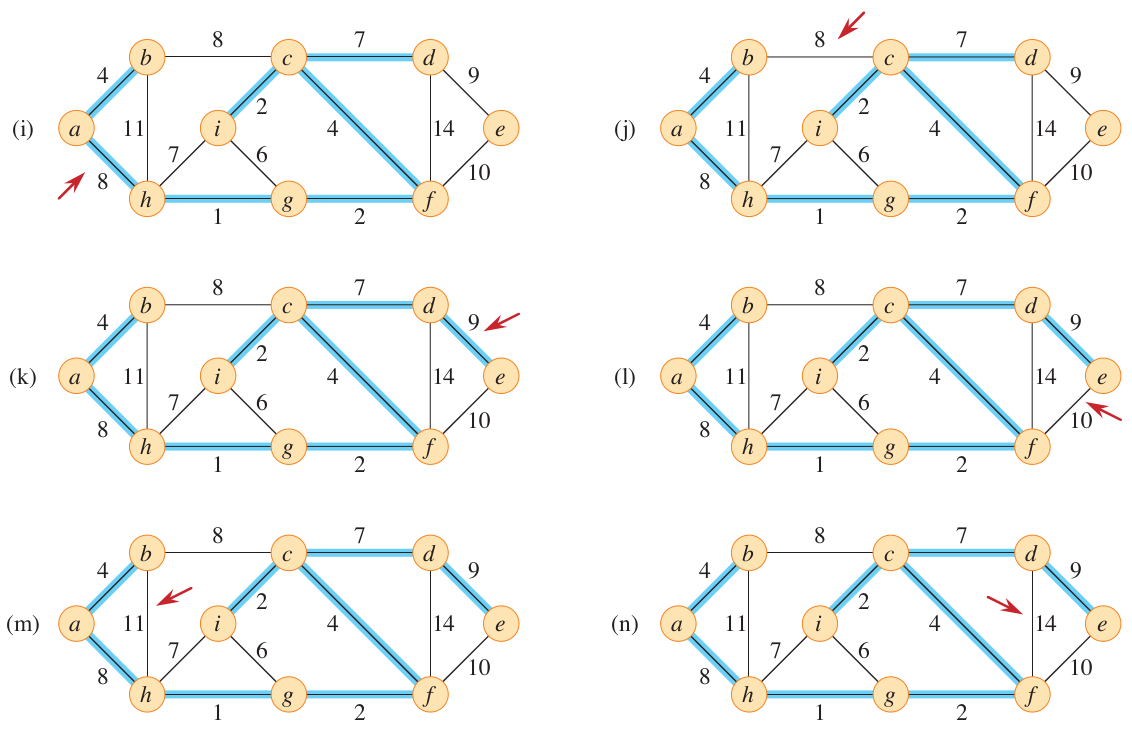
\includegraphics[width=0.7\textwidth]{figs/chap07/593-kruskal}
\end{figure}
\end{itemize}
\end{frame}


\begin{frame}{‌الگوریتم کروسکال}
\begin{itemize}\itemr
\item[-]
الگوریتم کروسکال در زیر نشان داده شده است.
\begin{algorithm}[H]\alglr
  \caption{Minimum Spanning Tree - Kruskal} 
  \begin{algorithmic}[1]
   \Func{Mst-Kruskal}{G,w}
   \State A = $\emptyset$
   \For{each vertex v $\in$ G.V}
   			\State Make-Set(v)
   	\EndFor
   	\State creat a single list of the edges in G.E
   	\State sort the list of edges into monotonically increasing order by weight w
   	\For{each edge(u,v) taken from the sorted list in order}
   			\If{Find-Set(u) $\neq$ Find-Set(v)}
   					\State A = A $\cup$ {(u,v)}
   					\State Union(Find-Set(u),Find-Set(v))
   			\EndIf
   	\EndFor
   	\State \Return A                           
  \end{algorithmic}
  \label{alg:merge}
\end{algorithm}
\end{itemize}
\end{frame}



\begin{frame}{‌الگوریتم کروسکال}
\begin{itemize}\itemr
\iffalse
\item[-]
مقدار دهی اولیه مجموعه
\m{A}
در زمان
\m{O(1)}
انجام می‌شود.
\item[-]
ساختن لیست یال‌ها در خط‌ ۴ در زمان
\m{O(V+E)}
انجام می‌شود. برای گراف همبند
\m{G}
این کار در
\m{O(E)}
انجام می‌شود.
\fi
\item[-]
در الگوریتم کروسکال،
زمان لازم برای مرتب‌سازی یال‌ها
\m{O(|E|lg|E|)}
است.
\item[-]
زمان لازم برای بررسی همهٔ یال‌ها
\m{O(|E|)}
است.
\item[-]
بنابراین، زمان اجرای الگوریتم کروسکال در مجموع
\m{O(|E|lg|E|)}
است.
\item[-]
همچنین با توجه به اینکه
\m{|E| < |V|^2}
، داریم
\m{lg|E| < 2lg|V|}
و بنابراین
\m{lg|E| = O(lg|V|)} .
پس می‌توانیم بگوییم زمان اجرای الگوریتم کروسکال برابراست با
\m{O(|E|lg|V|)} .
\end{itemize}
\end{frame}
